% A short paper about farleaf, used for the demo GIF and as a PDF to try it on.
% Build: pdflatex demo.tex (twice, for the outline).
\documentclass[12pt]{article}
\usepackage[margin=1.25in]{geometry}
\usepackage{lmodern}
\usepackage[T1]{fontenc}
\usepackage{amsmath}
\usepackage{booktabs}
\usepackage{tikz}
\usepackage{xcolor}
\usepackage[hidelinks,bookmarksnumbered,bookmarksopen]{hyperref}
\hypersetup{pdftitle={Reading PDFs in a Terminal}, pdfauthor={farleaf}}

\definecolor{c1}{HTML}{3B6EA8}
\definecolor{c2}{HTML}{C0603A}
\definecolor{c3}{HTML}{6A9A55}

\title{Reading PDFs in a Terminal,\\ Fast, Locally and over SSH}
\author{The farleaf project}
\date{October 2026}

\begin{document}
\maketitle

\begin{abstract}
\noindent
Terminals that speak the Kitty graphics protocol can show real images, which
makes reading a PDF without leaving the terminal practical. Doing it well is
mostly a matter of moving few bytes: a page is rendered once, sent in pieces,
and afterwards only moved. This note describes how farleaf does that, how it
picks the cheapest way to send an image, and how it stays inside the memory a
terminal is willing to spend on images. Page turns take a few hundredths of a
second locally and a few tenths over SSH.
\end{abstract}

\section{Introduction}

A PDF viewer in the terminal has an unusual constraint: everything it shows
travels through a pseudo-terminal, possibly over a network, possibly through a
multiplexer that keeps its own copy of the screen. A page rendered for a
high-resolution display is easily 25\,MB of pixels. Sent naively, as one image
per page turn, it would take seconds over SSH and exhaust the image memory of
some terminals after a handful of pages.

farleaf avoids most of that cost. It renders each page once, at exactly the
size of the cells it will cover, sends it in pieces, and from then on asks the
terminal to place images it already holds. The rest of this note explains the
three ideas behind that: pieces, transports, and a memory budget.

\subsection{What a reader needs}

Reading is mostly scrolling and turning pages, with the occasional jump: to a
section, a figure, a search hit. A viewer should make the common moves instant
and the rare ones quick. It should also never show a blank where a page
should be, which, as we will see, is the harder requirement.

\subsection{The terminals}

farleaf targets Ghostty and herdr, an agent multiplexer built on Ghostty's
terminal core. Both accept images over the Kitty graphics protocol. They differ
in how much image memory they keep: Ghostty about 320\,MB per screen, a herdr
pane only 64\,MiB.

\section{Design}

\subsection{Pages in pieces}

A page is cut into horizontal strips, and, when zoomed wider than the screen,
into tiles. A strip holds at most
\begin{equation}
  B_{\max} = 4\,\text{MB} \quad\text{and}\quad
  h_{\max} = \max\!\left(2, \left\lfloor \tfrac{R}{8} \right\rfloor\right)
  \text{ rows},
\end{equation}
where $R$ is the number of rows on screen. Small pieces keep every image under
the terminals' limits (10\,000 pixels on a side, 30\,MiB once encoded), let the
first strips show before the rest are rendered, and let a scroll move images
instead of sending them again.

\subsection{Choosing a transport}

At startup farleaf asks the terminal one question with several parts: can it
read shared memory on this machine, how big is a cell, and what is it. The
answers decide how images travel (Table~\ref{tab:transports}).

\begin{table}[h]
  \centering
  \begin{tabular}{lll}
    \toprule
    Where & Transport & Bytes per page \\
    \midrule
    Ghostty, same machine & shared memory & a few names \\
    Ghostty over SSH & PNG & 0.3--1\,MB \\
    herdr, local or remote & zlib RGB & 0.5--1\,MB \\
    \bottomrule
  \end{tabular}
  \caption{How images reach the terminal.}
  \label{tab:transports}
\end{table}

\subsection{A memory budget}

A terminal that runs out of image memory evicts images, and an evicted strip
is a blank stripe on the page. farleaf therefore keeps its own account. If
$m_i$ is the memory piece $i$ takes in the terminal, it keeps
\begin{equation}
  \sum_{i \in \text{sent}} m_i \;\le\; M,
  \qquad M = \begin{cases}
    192\,\text{MiB} & \text{in Ghostty,}\\
    56\,\text{MiB} & \text{in herdr,}
  \end{cases}
\end{equation}
prefetching nearest-first until the budget is spent, and freeing the least
wanted images before sending a new one.

\section{Measurements}

\subsection{Setup}

A fake terminal runs farleaf in a pseudo-terminal, emulates each terminal's
limits, and checks after every key that the screen shows exactly what farleaf
drew, pixel for pixel. The SSH link is modelled at 9\,MB/s with 50\,ms round
trips and compression.

\subsection{Results}

Figure~\ref{fig:latency} shows the typical time from a key to a complete
screen. Locally, a page turn mostly re-places images that are already there.
Over SSH inside herdr, the time is dominated by herdr re-sending each new
image to the outer terminal uncompressed.

\begin{figure}[h]
  \centering
  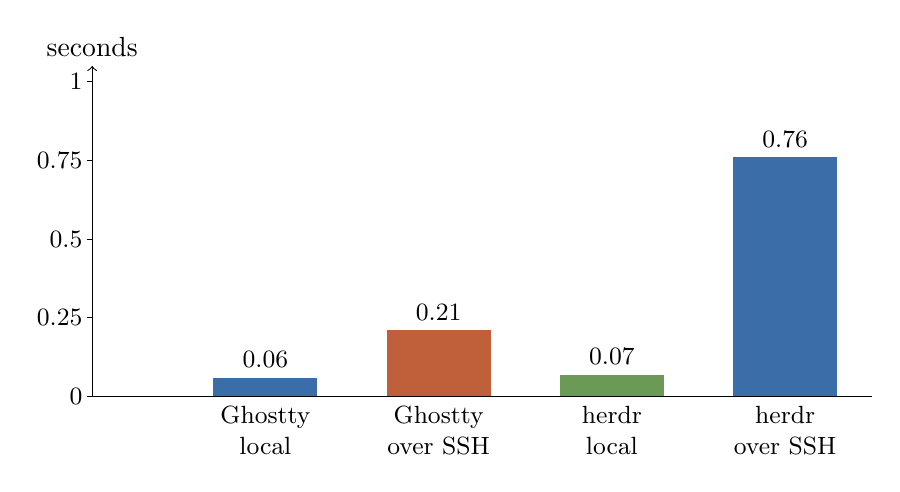
\begin{tikzpicture}[x=2.2cm, y=4cm]
    \draw[->] (0,0) -- (0,1.05) node[above] {seconds};
    \foreach \y in {0,0.25,0.5,0.75,1}
      \draw (-0.03,\y) -- (0,\y) node[left] {\small\y};
    \foreach \x/\v/\c/\l in {1/0.06/c1/{Ghostty\\local}, 2/0.21/c2/{Ghostty\\over SSH},
                             3/0.07/c3/{herdr\\local}, 4/0.76/c1/{herdr\\over SSH}}
    {
      \fill[\c] (\x-0.3,0) rectangle (\x+0.3,\v);
      \node[above] at (\x,\v) {\small\v};
      \node[below, align=center, font=\small] at (\x,0) {\l};
    }
    \draw (0,0) -- (4.5,0);
  \end{tikzpicture}
  \caption{Typical seconds from a page turn to a complete screen.}
  \label{fig:latency}
\end{figure}

\section{Navigation}

\subsection{The outline}

Most papers carry an outline: the sections and subsections, each pointing at a
place on a page. farleaf lists it in a sidebar; moving through the list shows
each place as you go, Enter stays there, and Escape returns to where you were.

\subsection{Thumbnails}

The other sidebar shows a small image of every page, as a desktop viewer does.
Thumbnails are images like any other: they count against the same budget, are
prefetched a few pages ahead, and are kept across zooms and resizes when their
size does not change.

\section{Implementation}

\subsection{Two threads}

pdfium, the renderer, is not thread-safe, so a single worker thread owns it.
The worker renders strips in the order the main thread asks for them: what is
on screen first, then the rest of the page, then the next two pages and the
previous one. When the reader moves on, the queue is replaced, and strips that
are no longer wanted are never rendered.

A second thread owns the terminal. Small frames, which place images and draw
the status line, jump ahead of queued uploads, so a key always gets an answer
within one frame even while a large image is still on its way over a slow
link. Uploads that stop being wanted while they wait are dropped before they
are sent.

\subsection{Reloading}

Writing a paper usually means rebuilding the PDF many times. farleaf polls the
file twice a second and reloads it once it has stopped changing, so a LaTeX
run is read when it is done rather than halfway. The document is read into
memory first, so a rebuild cannot change what is on screen underneath the
reader. The reading position is kept: after a rebuild, the same paragraph is
still on screen.

\subsection{Search}

Search runs on the worker too, page by page from the current one, and stops
at the first page with a match. Matches are painted into the strips that
contain them, like a highlighter pen: the paper turns yellow and the ink stays
dark. Clearing the highlights re-renders only the strips that had any.

\section{Limits}

Some things are left out on purpose. Text cannot be selected, the mouse is not
used, and tmux, which needs extra setup to pass images through, is not
supported. Each of these would be useful, and each would add code that has to
stay fast over a slow link. The guiding rule is that a feature has to earn its
place by making reading better.

\section{Conclusion}

Fast terminal graphics are less about fast rendering than about sending
little. Rendering at the size of the cells, cutting pages into pieces, asking
the terminal what it can do, and respecting its memory make a PDF viewer that
feels local even when the document is on the other side of an SSH connection.

\appendix
\section{Keys}

\begin{center}
  \begin{tabular}{ll}
    \toprule
    Keys & Action \\
    \midrule
    \texttt{j} \texttt{k} & scroll \\
    \texttt{l} \texttt{h} & next / previous page \\
    \texttt{gg} \texttt{G} & first page / end \\
    \texttt{z} \texttt{Z} & fit page / fit width \\
    \texttt{/} \texttt{n} \texttt{N} & search, next / previous match \\
    \texttt{o} & outline \\
    \texttt{t} & page thumbnails \\
    \texttt{?} & every key \\
    \texttt{q} & quit \\
    \bottomrule
  \end{tabular}
\end{center}

\end{document}
